\chapter{CArt-OnePiece}

CArt-OnePiece was conceived as a generic and extensible framework for the applications of autonomous driving vehicles. Its design allows multiple sensor configurations, processing modules, flexible synthetic dataset generation, and alternative scheduling policies to be incorporated into the same execution environment. It enables the framework to be used not only as an application pipeline, but also as an experimental instrument for studying workload behavior, algorithm training via datasets, and task scheduling in heterogeneous computing environments.

To organize this discussion, the chapter begins by presenting a global view of the pipeline and its main stages. Subsequently, the following sections detail the modules and mechanisms that compose the framework, emphasizing how the different components interact to support both workload execution and experimental evaluation.

\section{Pipeline Overview}

Figure~\ref{fig:cart_onepiece_pipeline} presents an overview of the CArt-OnePiece pipeline. At a high level, the framework is organized as a sequence of stages that begins with the configuration of the simulation environment, proceeds through sensor data acquisition and workload execution, and culminates in the production of outputs for performance analysis and synthetic dataset generation. In addition to this central flow, the framework also allows the incorporation of user-defined scheduling strategies and user-defined processing modules.

\begin{figure}[H]
  \setlength{\abovecaptionskip}{0pt} \setlength{\belowcaptionskip}{0pt}
  \caption{\MakeUppercase{System Overview}}
  \centering
  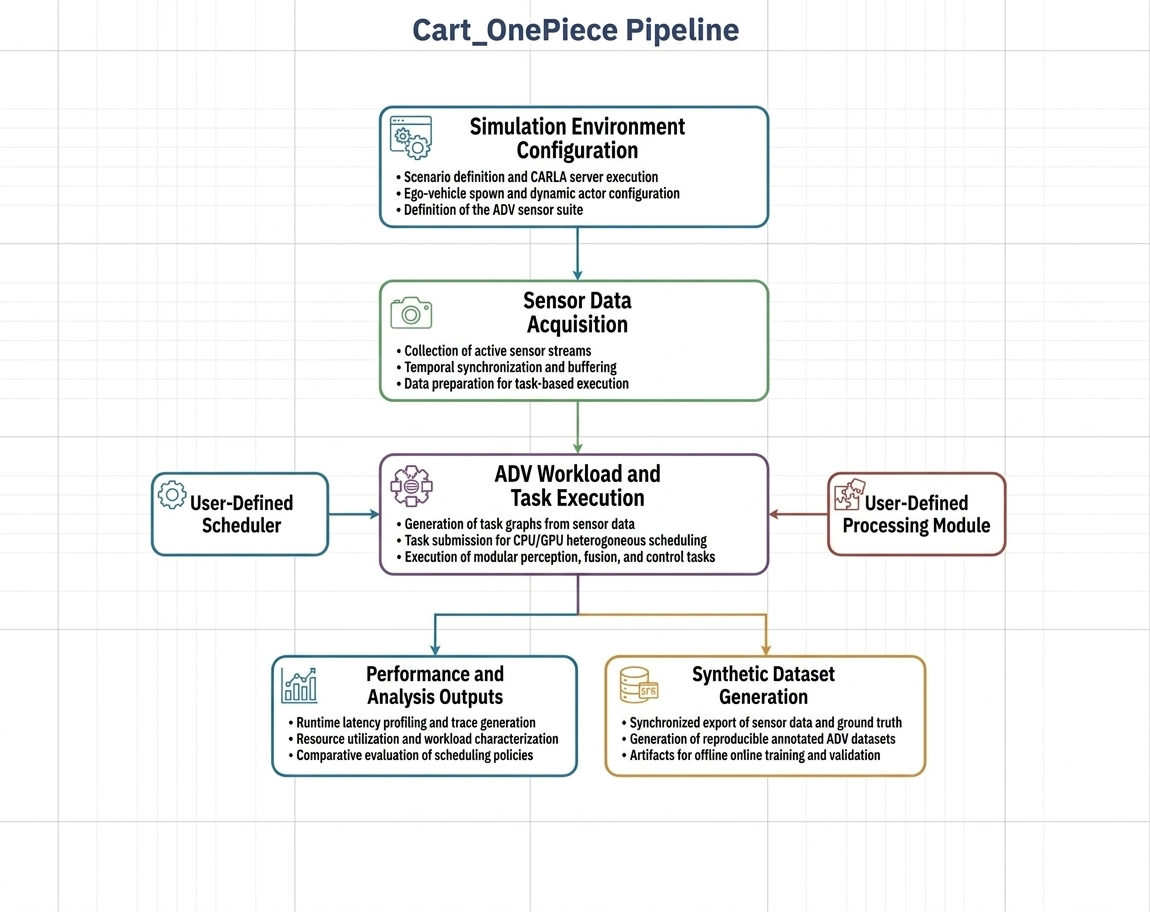
\includegraphics[width=1\textwidth]{imagens/Cart_OnePiece_Pipeline.png}
  \captionsetup{justification=centering}
  \captionfont{\small{\textbf{\\Source: Elaborated by the author}}}  
  \label{fig:cart_onepiece_pipeline}
\end{figure}

The first stage of the pipeline corresponds to the configuration of the simulation environment. In this stage, the virtual scenario is defined, the CARLA server is executed, and the ego vehicle and dynamic actors are instantiated according to the requirements of the experiment. This stage also includes the definition of the vehicle-associated sensor suite, which can be adapted to the needs of different autonomous driving workloads.

Once the scenario is configured, the pipeline advances to sensor data acquisition. At this stage, the framework manages the collection of active sensor streams, which may encompass a wide range of sensor types ranging from multiple RGB cameras and semantic sensors to LiDAR and Radar data. The pipeline also handles the temporal synchronization and buffering of these heterogeneous streams, preparing the raw data for task-based execution.

The next stage corresponds to the ADV workload and task execution, which constitutes the central processing core of the framework.  At this point, the framework uses the StarPU runtime system to encapsulate the core ADV operations into computational tasks and submit them for CPU/GPU heterogeneous scheduling. An important characteristic of this stage is that it also supports external customization through user-defined schedulers and user-defined processing modules.

User-defined processing modules allow for the execution of generic perception, fusion, planning, or control tasks. At the same time, the framework also supports user-defined schedulers, providing the flexibility to determine how these generic ADV tasks are distributed across available hardware resources and enabling the evaluation of different scheduling policies.

The output of the framework is divided into two main branches. The first branch comprises performance and analysis output, including latency measurements, execution traces, workload characterization artifacts, and comparative scheduling results. The second branch corresponds to the generation of synthetic datasets, in which sensor data and associated ground-truth information can be exported and organized as reusable artifacts for later training, validation, or complementary experiments.

The following subsections describe in detail each of the stages that make up the Cart-OnePiece framework.